\pdfminorversion=7 %added to avoid warning about pdf versions
%note Non-PDF special ignored! warning may be related to the .cls using ps commands somewhere.
\documentclass[12pt,letterpaper]{article}


%%%%%%%%%%%BEGIN SYS BIO COMMANDS %%%%%%%%%%%%
%%Taken from SB_LaTeX_Template.tex provided by OUP
%% that file is almost identical to the version found on overleaf website.
%\usepackage{bibtex}
%\usepackage{html}
%\usepackage{hyperref} 
%\usepackage{nag}
%\usepackage{xcolor}
\usepackage[english]{babel}
\usepackage[normalem]{ulem}
\usepackage{amsfonts}
\usepackage{amsmath}
\usepackage{amssymb}
\usepackage{amstext}
\usepackage{amsthm}
\usepackage{array}
\usepackage{bm}
\usepackage{booktabs}
\usepackage{caption}
\usepackage{color}
%\usepackage{epsfig}
\usepackage{fixltx2e}
\usepackage{float}
\usepackage{fullpage}
\usepackage{graphicx}
\usepackage{hyperref}
\usepackage{hyperref}
\usepackage{ifthen}
\usepackage{indentfirst}
\usepackage{latexsym}
\usepackage{lscape}
%\usepackage{mhchem}
\usepackage{natbib}
\usepackage{pifont}
\usepackage{setspace}
\usepackage{textcomp}
\usepackage{url}
\usepackage{verbatim}


\linespread{1.66}
% All text should be double-spaced
% with occasional exceptions for tables. 
\raggedright
\setlength{\parindent}{0.5in}

\setcounter{secnumdepth}{0}
% Our sections are not numbered and our papers do not have
% Tables of Contents. We don't 
% present a list of figures or list of tables, either.

% Any common font is fine.
% (A common sans-serif font should be used on figures, but figures should be
% separate from the LaTeX document.)

\pagestyle{empty}

\renewcommand{\section}[1]{%
\bigskip
\begin{center}
\begin{Large}
\normalfont\scshape #1
\medskip
\end{Large}
\end{center}}

\renewcommand{\subsection}[1]{%
\bigskip
\begin{center}
\begin{large}
\normalfont\itshape #1
\end{large}
\end{center}}

\renewcommand{\subsubsection}[1]{%
\vspace{2ex}
\noindent
\textit{#1.}---}

\renewcommand{\tableofcontents}{}

\bibpunct{(}{)}{;}{a}{}{,}  % this is a citation format command for natbib

%%%%%%%%%%%END SYS BIO COMMANDS %%%%%%%%%%%%


%\usepackage[doublespacing]{setspace}
%\usepackage[nomarkers,figuresonly]{endfloat}  %%place all figures at end
%\usepackage{amsmath, amssymb,amsfonts}
%\usepackage{fullpage} %this causes problems with the sysbio style file
%\usepackage[normalem]{ulem} %strike out via \sout{}
%\usepackage[small]{caption}
\usepackage{datetime} %provides \currenttime command
%\usepackage{float}
%\usepackage{graphicx}
%\usepackage{natbib}
\usepackage{subfig}
%\usepackage{url}
\usepackage{xspace}

\graphicspath{{./Figures/}} \DeclareGraphicsExtensions{.pdf, .jpg, .png}



%%%%%%%%%%%%%%%%%%%%%%%%%%%%%%%%%Local Commands%%%%%%%%%%%%%%%%%%%%%%%%%%%%%
%%% Sort using M-x 'sort-lines'
\newcommand{\Costaobsvec}{\ensuremath{\Cost(\aobsvec)}\xspace}
\newcommand{\Costaveci}{\ensuremath{\Cost(\aveci)}\xspace}
\newcommand{\Costavecj}{\ensuremath{\Cost(\avecj)}\xspace}
\newcommand{\Costavec}{\ensuremath{\Cost(\avec)}\xspace}
\newcommand{\Costcveci}{\ensuremath{\Cost(\cveci)}\xspace}
\newcommand{\Costcvecj}{\ensuremath{\Cost(\cvecj)}\xspace}
\newcommand{\Cost}{\ensuremath{\text{\textbf{C}}}\xspace}
\newcommand{\DeltaAIC}{\ensuremath{\Delta\text{AIC}}\xspace}
\newcommand{\AICw}{\ensuremath{\text{AIC}_\text{w}}\xspace}
\newcommand{\EE}{\mathbb{E}} %use for expectation function E()
\newcommand{\Funcaobsvec}{\ensuremath{\Func(\aobsvec|\aoptvec)}\xspace}
\newcommand{\Funcaoptvec}{\ensuremath{\Func(\aoptvec)}\xspace}
\newcommand{\Funcaveci}{\ensuremath{\Func(\aveci|\aoptvec)}\xspace}
\newcommand{\Funcavecj}{\ensuremath{\Func(\avecj|\aoptvec)}\xspace}
\newcommand{\Funcavec}{\ensuremath{\Func(\avec|\aoptvec)}\xspace}
\newcommand{\Funccveci}{\ensuremath{\Func(\cveci|\aoptvec)}\xspace}
\newcommand{\Funccvec}{\ensuremath{\Func(\cvec|\aoptvec)}\xspace}
\newcommand{\Func}{\ensuremath{\text{\textbf{B}}}\xspace}
\newcommand{\GTR}{GTR+$\Gamma$\xspace}
\newcommand{\LogN}{\ensuremath{\text{LogN}}\xspace}
\newcommand{\Ne}{\ensuremath{{N_e}}\xspace} %
\newcommand{\Nemu}{\ensuremath{{N_e \mu}}\xspace} %
\newcommand{\Lik}{\ensuremath{\mathcal{L}}\xspace}%replaces \Lmatrix which was inconsistent and, thus, confusing 
\newcommand{\pimatrix}{\ensuremath{\mathbf{\pi}}\xspace}
\newcommand{\mumatrix}{\ensuremath{\mathbf{\mu}}\xspace}
\newcommand{\Pmatrix}{\ensuremath{\mathbf{P}}\xspace}
\newcommand{\Tmatrix}{\ensuremath{\mathbf{T}}\xspace}
\newcommand{\Dmatrix}{\ensuremath{\mathbf{D}}\xspace}
\newcommand{\Dmatrixp}{\ensuremath{\mathbf{D}_p}\xspace}
\newcommand{\Mmatrix}{\ensuremath{\mathbf{M}}\xspace}
\newcommand{\Qmatrix}{\ensuremath{\mathbf{Q}}\xspace}
\newcommand{\Qmatrixa}{\ensuremath{\Qmatrix_a}\xspace}
\newcommand{\Wi}{\ensuremath{{W_i}}\xspace}
\newcommand{\Wj}{\ensuremath{{W_j}}\xspace}
\newcommand{\simP}{\ensuremath{\sim P}\xspace}
\newcommand{\selac}{SelAC\xspace}
\newcommand{\selacplusgamma}{SelAC$+\Gamma$\xspace}
\newcommand{\acivec}{\ensuremath{a\left(\cveci\right)}\xspace}
\newcommand{\acvecg}{\ensuremath{a\left(\vec{c}_{i,g}\right)}\xspace}
\newcommand{\acvecj}{\ensuremath{a\left(\cvecj\right)}\xspace}
\newcommand{\acvec}{\ensuremath{a\left(\Vec{c}\right)}\xspace}
\newcommand{\aip}{\ensuremath{a_{i,p}}\xspace}
\newcommand{\aivecg}{\ensuremath{{\avec}_{i,g}}\xspace}
\newcommand{\aivec}{\aveci}
\newcommand{\ajp}{\ensuremath{a_{j,p}}\xspace}
\newcommand{\ajvecg}{\ensuremath{{\ajvec}_{,g}}\xspace}
\newcommand{\ajvec}{\ensuremath{\Vec{a}_{j}}\xspace}
\newcommand{\aj}{\ensuremath{a__j}\xspace}
\newcommand{\alphac}{\ensuremath{\alpha_c}\xspace}
\newcommand{\alphag}{\ensuremath{\alpha_G}\xspace}
\newcommand{\alphap}{\ensuremath{\alpha_p}\xspace}
\newcommand{\alphavec}{\ensuremath{\Vec{\alpha}}\xspace}
\newcommand{\alphav}{\ensuremath{\alpha_v}\xspace}
\newcommand{\alphavValue}{\ensuremath{4 \times 10^{-4}}\xspace}
\newcommand{\aobsvecg}{\ensuremath{{\avec}_{\text{obs},g}}\xspace}
\newcommand{\aobsvec}{\ensuremath{\Vec{a}_{\text{obs}}}\xspace}
\newcommand{\aobs}{\ensuremath{a_{\text{obs}}}\xspace}
\newcommand{\aopt}{\ensuremath{a_*}\xspace}
\newcommand{\aoptip}{\ensuremath{\aopt_{i,p}}\xspace}
\newcommand{\aoptpg}{\ensuremath{\aopt_{p,g}}\xspace}
\newcommand{\aoptp}{\ensuremath{a_{*,p}}\xspace}
\newcommand{\aoptvecg}{\ensuremath{{{\aoptvec}_g}}\xspace}
\newcommand{\aoptvec}{\ensuremath{\Vec{a}_*}\xspace}
\newcommand{\aveci}{\ensuremath{\Vec{a}_i}\xspace}
\newcommand{\avecj}{\ensuremath{\Vec{a}_j}\xspace}
\newcommand{\avec}{\ensuremath{\Vec{a}}\xspace}
\newcommand{\cveci}{\ensuremath{\cvec_i}\xspace}
\newcommand{\cvecj}{\ensuremath{\cvec_j}\xspace}
\newcommand{\cvec}{\ensuremath{\Vec{c}}\xspace}
\newcommand{\deltaT}{\ensuremath{\delta t}\xspace}
\newcommand{\etag}{\ensuremath{\eta_g}\xspace}
\newcommand{\fij}{\ensuremath{f_{i,j}}\xspace}
\newcommand{\jmax}{\ensuremath{{j_{\max}}}\xspace}
\newcommand{\kmax}{\ensuremath{{k_{\max}}}\xspace}
\newcommand{\muij}{\ensuremath{\mu_{i,j}}\xspace}
\newcommand{\muvec}{\ensuremath{\Vec{\mu}}\xspace}
\newcommand{\phig}{\ensuremath{\phi_{g}}\xspace}
\newcommand{\phiprime}{\ensuremath{\phi^\prime}\xspace}
\newcommand{\psig}{\ensuremath{\psi_{g}}\xspace}
\newcommand{\psiprime}{\ensuremath{\psi^\prime}\xspace}
\newcommand{\pij}{\ensuremath{p_{i,j}}\xspace}
\newcommand{\qij}{\ensuremath{q_{i,j}}\xspace}
\newcommand{\qji}{\ensuremath{q_{i,j}}\xspace}
\newcommand{\setG}{\ensuremath{\mathbb{G}}\xspace}
\newcommand{\setP}{\ensuremath{\mathbb{P}}\xspace}
\renewcommand{\ng}{\ensuremath{{n_g}}\xspace}
\newcommand{\gp}{\ensuremath{{G_p}}\xspace}
\DeclareMathOperator{\Var}{Var}

\date{Last compiled on \today\xspace at \currenttime.}

\begin{document}
\title[BEAULIEU ET AL.--- Pop. Gen. Based Phylo.]{Population Genetics Based Phylogenetics Under Stabilizing Selection for an Optimal Amino Acid Sequence: A Nested Modeling Approach}

\author[]{J\textsc{EREMY} M.~{B\textsc{EAULIEU}}$^{1,2,3}$,
J\textsc{UAN JUAN} {C\textsc{ROSSKEY}}$^{2,4}$
C\textsc{EDRIC} {L\textsc{ANDER}}$^{2,3}$, 
R\textsc{USSELL} {Z\textsc{ARETZKI}}$^{5}$, 
B\textsc{RIAN} C.~{O'\textsc{MEARA}}$^{2,3}$, 
\textsc{AND}
M\textsc{ICHAEL} A.~{G\textsc{ILCHRIST}}$^{2,3\ast}$}

\noindent {\small $^1$Department of Biological Sciences, University of Arkansas, Fayetteville, AR 72701
$^{2}$Department of Ecology \& Evolutionary Biology, University of Tennessee, Knoxville, TN 37996-1610
$^{3}$National Institute for Mathematical and Biological Synthesis, Knoxville, TN 37996-3410
$^{4}$JJ's Address
$^{5}$Department of Business Analytics \& Statistics, Knoxville, TN ~ 37996-0532 
$^{\ast}$Correspondence to be sent to: Michael A. Gilchrist, 569 Dabney Hall, University of Tennessee, Knoxville TN 37996-1610\\
E-mail:~mikeg@utk.edu
}

%%FROM SB_.. .tex file
%\begin{flushright}
%Version dated: \today
%\end{flushright}
%\bigskip
%\noindent RH:  A LATEX FORMATTING TEMPLATE FOR SYSTEMATIC
%  BIOLOGY
%% put in your own RH (running head)
%% for POVs the RH is always POINT OF VIEW
%
%\bigskip
%\medskip
%

%\history{Compiled \today; Submitted DAY-March-2017}


\abstract{
We present a phylogenetic approach rooted in the field of population genetics that more realistically models the evolution of protein-coding DNA under the assumption of stabilizing selection for a gene specific optimal amino acid sequence.
The new set of models, which we collectively call SelAC models, fit phylogenetic data substantially better than popular models, suggesting strong potential for more accurate inference of phylogenetic trees and branch lengths.
Moreover, these models allow inference of population genetics parameters from data used for interspecific phylogenies.
}

\maketitle 

%\section{Introduction}
Phylogenetic analysis now plays a critical role in most aspects of biology, particularly in the fields of ecology, evolution, paleontology, medicine, and conservation.
While the scale and impact of phylogenetic studies has increased substantially over the past two decades, by comparison the realism of the mathematical models on which these analyses are based has changed relatively little.
For example, the simplest but most popular models are agnostic with regards to the different amino acid substitutions and their impact on gene function (e.g.~F81, F84, HYK85, TN93, and GTR, see \citet{Yang2014} for an overview).

Another set of models attempt to include a 'selection' term $\omega$, but the link between $\omega$ and the key parameters found in standard population genetics models such as \Ne, the distribution of fitness across genotype space, and mutation bias are far from clear.
For instance, $\omega$ is generally interpreted as indicating whether a sequence is under `purifying' ($\omega < 1$) or `diversifying' ($\omega > 1$) selection.
However, the actual behavior of the model as is quite different.
When $\omega < 1$ the model behaves as if the resident amino acid $i$ at a given site is favored by selection since synonymous substitutions have a higher substitution rate than any possible non-synonymous substitutions.
Paradoxically, this selection regime for the resident amino acid $i$ persists \emph{until} a substitution for another amino acid, $j$, occurs.
As soon as amino acid $j$ fixes, but not before, selection now favors amino acid $j$ over all other amino acids, including $i$.
This is now the opposite scenario to when $i$ was the resident.
Similarly, when $\omega > 1$, synonymous substitutions have a lower substitution rate than any possible non-synonymous substitutions the resident amino acid.
In a parallel manner, this selection \emph{against} the resident amino acid $i$ persists until a substitution occurs at which point selection now \emph{favors} the former resident amino acid $i$ as well as the 18 others.
Thus, the simplest and most consistent interpretation of $\omega$ is that it describes the rate at which the selection regime itself changes, and this change in selection perfectly coincides with the fixation of a new amino acid.
As a result, $\omega$ based approaches only reasonably describe a subset of scenarios such as over/underdominance or frequency dependent selection \citep{HughesAndNei1988,Nowak2006}.
Because, as we show here, $\omega$ is well correlated with gene expression, its value is really an indicator of the strength of stabilizing selection on a coding sequence, rather than the 'nature' of that selection.

Fortunately, given the continual growth in computational power available to researchers, it is now possible to utilize a more general set of population genetics based models for the purpose of phylogenetic analysis \citep[e.g.][]{HalpernAndBruno1998,RobinsonEtAl2003,LartillotAndPhilippe2004,RodrigueAndLartillot2014}.
One lesson from the field of population genetics is even when there are only a few fundamental evolutionary forces at play (mutation, drift, selection, and linkage effects), describing the evolutionary behavior of a system in which there are non-linear interactions between sites, such as epistasis, quickly becomes extremely challenging.
Fortunately, under the simplifying assumptions of additivity between sites and alleles, calculating stationary and substitution probabilities are relatively straightforward, making fitting additive models of the evolutionary process to sequence data computationally feasible.

\section{Materials \& Methods}

\subsection{Overview}

We model the substitution process as a classic Wright-Fisher process which includes the forces of mutation, selection, and drift \citep{Fisher1930,Kimura1962,Wright1969,Iwasa1988,BergAndLassig2003,SellaAndHirsh2005,McCandlishAndStoltzfus2014}.
For simplicity, we ignore linkage effects and, as a result of this and other assumptions, our method behaves in a site independent manner.
Our approach, which we call \selac (Selection on Amino acids and Codons), is developed in the same vein as previous phylogenetic applications of the Wright-Fisher process \citep[e.g.][]{MuseAndGaut1994,HalpernAndBruno1998,YangAndNielsen2008,RodrigueEtAl2005,KoshiAndGoldstein1997,KoshiEtAl1999,DimmicEtAl2000,ThorneEtAl2012,LartillotAndPhilippe2004,RodrigueAndLartillot2014}.
Similar to Lartillot's work \citep{LartillotAndPhilippe2004,RodrigueAndLartillot2014}, we assume there is a finite set of rate matrices describing the substitution process and that each position within a protein is assigned to a particular rate matrix category.
Unlike this previous work, we assume \emph{a priori} there are 20 different families of rate matrices, one family for when a given amino acid is favored at a site.
As a result, \selac allows us to quantitatively evaluate the support for a particular amino acid being favored at a particular position within the protein encoded by a particular gene.

Because \selac requires twenty families of $61 \times 61$ matrices, the number of parameters needed to implement \selac would, without further assumptions, be extremely large.
To reduce the number of parameters needed while still maintaining a high degree of biological realism, we construct our gene and amino acid specific substitution matrices using a submodel nested within our substitution model, similar to approaches in \citet{Gilchrist2007,ShahAndGilchrist2011,GilchristEtAl2015}.

One advantage of a nested modeling framework is that it requires only a handful of genome wide parameters such as nucleotide specific mutation rates (scaled by effective population size \Ne), side chain physicochemical weighting parameters, and a shape parameter describing the distribution of site sensitivities. % around a mean value of 1.
In addition to these genome wide parameters, \selac requires a gene $g$ specific expression parameter $\psi_g$ which describes the average rate at which the protein's functionality is produced by the organism.
Currently, $\psi$ is fixed across the phylogeny, though relaxing this assumption is a goal of future work.
The gene specific parameter $\psi_g$ is multiplied by additional model terms to make a composite term $\psiprime_g$ which scales the strength and efficacy of selection for the optimal amino acid sequence relative to drift.
In terms of the functionality of the protein encoded, we assume that for any given gene there exists an optimal amino acid sequence \aoptvec and that, by definition, a complete, error free peptide consisting of \aopt provides one unit of the gene's functionality.
We also assume that natural selection favors genotypes that are able to synthesize their proteome efficiently than their competitors and that each savings of an high energy phosphate bond per unit time leads to a constant proportional gain in fitness $q$.
\selac also requires the specification (as part of parameter optimization) of an optimal amino acid at each position or site within a coding sequence which, in turn, makes it the largest category of parameters we estimate.
Because we use a submodel to derive our substitution matrices, \selac requires the estimation of a fraction of the parameters required when compared to approaches where the substitution rates are allowed to vary independently \citep{HalpernAndBruno1998,LartillotAndPhilippe2004,RodrigueAndLartillot2014}.

As with other phylogenetic methods, we generate estimates of branch lengths and nucleotide specific mutation rates.
In addition, because the math behind our model is mechanistically derived, our method can also be used to make quantitative inferences on the optimal amino acid sequence of a given protein as well as the average synthesis rate of each protein used in the analysis.
The mechanistic basis of \selac also means it can be easily extended to include more biological realism and test more explicit hypotheses about sequence evolution.

\subsection{Mutation Rate Matrix \mumatrix}
We begin with a 4x4 nucleotide mutation matrix that defines a model for mutation rates between individual bases.
For our purposes, we rely on the general unrestricted model\citep[UNREST]{Yang1994} because it makes no constraint on the instantaneous rate of change between any pair of nucleotides.
We note, however, that more constrained models, such as the Jukes-Cantor (JC), Hasegawa-Kishino-Yano (HKY), or the general time reversible model (GTR), can also be used.
The 12 parameter UNREST model defines the relative rates of change between a pair of nucleotides.
Thus, we arbitrarily set the G$\rightarrow$T mutation rate to 1, resulting in 11 free mutation rate parameters in the 4x4 mutation nucleotide mutation matrix.
The nucleotide mutation matrix is also scaled by a diagonal matrix \pimatrix whose entries correspond to the equilibrium frequencies of each base.
These equilibrium nucleotide frequencies are determined by analytically solving $\pimatrix \times \Qmatrix = 0$. 
We use this \Qmatrix to populate a $61 \times 61$ codon mutation matrix $\mumatrix$, whose entries $\muij$ describe the mutation rate from codon $i$ to $j$ under a "weak mutation" assumption.
That is, the rate of allele fixation is much greater than \Nemu and $\Nemu \ll 1$, such that evolution is mutation limited, codon substitutions only occur one nucleotide at a time and, as a result, the rate of change between any pair of codons that differ by more than one nucleotide is zero.

While the overall model does not assume equilibrium, we still need to scale our mutation matrices $\mu$.
Traditionally, it is rescaled such that at equilibrium, one unit of branch length represents one expected substitution per site.
Here, a scaling factor is calculated as the average rate $-\sum_i \mu_i \pi_i=1$, where $i$ indexes a particular codon in a given gene.
The final mutation rate matrix is the original mutation rate matrix multiplied by 1/scaling factor.

\subsection{Protein Synthesis Cost-Benefit Function $\eta$}
\selac links fitness to the product of the cost-benefit function of a gene $g$, $\etag$, and the organism's average target synthesis rate of the functionality provided by gene $g$, $\psig$.
This is because the average flux energy an organism spends to met its target functionality provided by gene $g$ is $\etag \times \psig$.
In order to link genotype to our cost-benefit function $\eta = \Func/\Cost$, we begin by defining our benefit function \Func.

\subsubsection{Benefit:}
Our benefit function \Func measures the functionality of the amino acid sequence \aveci encoded by a set of codons \cveci, i.e. $a(\cveci) = \aveci$ relative to that of an optimal sequence $\aoptvec$.
By definition, $\Funcaoptvec = 1$ and $\Funcaveci < 1$ for all other sequences.
We assume all amino acids within the sequence contribute to protein function and that this contribution declines as an inverse function of physicochemical distance between each amino acid and the optimal.
Formally, we assume that
\begin{equation}
\Funcaveci = \left(\frac{1}{\ng} \sum_{p=1}^\ng \left(1 + \gp d(\aip, \aoptp\right)\right)^{-1}
\end{equation}
where $\ng$ is the length of the protein, $d(\aip, \aoptp)$ is a weighted physicochemical distance between the amino acid encoded in gene $i$ for position $p$ and $\aoptp$ is the optimal amino acid for that position of the protein.
For simplicity, we define the distance between a stop codon and a sense codon as effectively infinite and, as a result, nonsense mutations are effectively lethal. %% B/C it's a VERY BIG number, not Inf, correct?
The term \gp describes the sensitivity of the protein's function to deviation in physicochemical space.
There are many possible measures for physiochemical distance; we use \citep{Grantham1974} distances by default, though others may be chosen. 
We assume that $\gp \sim \text{Gamma}\left(\alpha = \alphag, \beta = \alphag\right)$ in order to ensure $\EE(\gp) = 1$.

At the limit of $\alphag \rightarrow \infty$, the model collapses to a model with uniform sensitivity of $\gp = 1$ for all positions $p$.
\Funcaveci is inversely proportional to the average physicochemical deviation of an amino acid sequence \aveci from the optimal sequence \aoptvec weighted by each sites senstivity to this deviation.
\Funcaveci can be generalized to include second and higher order terms of the distance measure $d$.


\subsubsection{Cost:}
Protein synthesis involves both direct and indirect assembly costs.
Direct costs consist of the high energy phosphate bonds \simP of ATP or GTP's used to assemble the ribosome on the mRNA, charge tRNA's for elongation, move the ribosome forward along the transcript, and terminate protein synthesis.
As a result, direct protein assembly costs are the same for all proteins of the same length.
Indirect costs of protein assembly are potentially numerous and could include the cost of amino acid synthesis as well the cost and efficiency with which the protein assembly infrastructure such as ribosomes, aminoacyl-tRNA synthetases, tRNAs, and mRNAs are used.
When these indirect costs are combined with sequence specific benefits, the probability of a mutant allele fixing is no longer independent of the rest of the sequence \citep{GilchristEtAl2015} and, as a result, model fitting becomes substantially more complex.
Thus for simplicity, in this study we ignore any indirect costs of protein assembly that vary between genotypes and define,
\begin{align}
\label{eq:defineCost}
  \Costcveci  &= \text{Energetic cost of protein synthesis.}\\
  &= A_1 + A_2 n
\end{align}
where, $A_1$ and $A_2$ represent the direct cost, in high energy phosphate bonds, of ribosome initiation and peptide elongation, respectively, where $A_1 = A_2 = 4  \, \simP$.


\subsection{Defining Physicochemical Distances}
Assuming that functionality declines with an amino acid $a_i$'s physicochemical distance from the optimum amino acid \aopt at each site provides a biologically defensible way of mapping genotype to protein function that requires relatively few free parameters.
In addition, \selac naturally lends itself to model selection since we can compare the quality of \selac fits using different mixtures of physicochemical properties.
Following \cite{Grantham1974}, we focus on using composition $c$, polarity $p$, and molecular volume $v$ of each amino acid's side chain residue to define our distance function, but the model and its implementation can flexibly handle a variety of properties.
We use the Euclidian distance between residue properties where each property $c$, $p$, and $v$ has its own weighting term, $\alphac$, $\alphap$, $\alphav$, respectively, which we refer to as `Grantham weights'.
Because physicochemical distance is ultimately weighted by a gene's specific average protein synthesis rate $\psi$, another parameter we estimate, there is a problem with parameter identifiablity.
Ultimately, the scale of gene expression is affected by how we measure physicochemical distances which, in turn, is determined by our choice of Grantham weights.
As a result, by default we set $\alphav = 3.990 \times 10^{-4}$, the value originally estimated by Grantham, and recognize that our our estimates of $\alphac$ and $\alphap$ and $\psi$ are scaled relative to this choice for $\alphav$.
More specifically,
\begin{align*}
  d(a_i, \aopt) &= \left(\alphac \left(c\left(a_i\right) - c\left(\aopt\right)\right)^2 + \alphap \left(p\left(a_i\right) - p\left(\aopt\right)\right)^2 + \right.\\
  & \;\;\;\;\;\left. \alphav \left(v\left(a_i\right) - v\left(\aopt\right)\right)^2\right)^{1/2}.
\end{align*}


\subsection{Linking Protein Synthesis to Allele Substitution}
Next we link the protein synthesis cost-benefit function $\eta$ of an allele with its fixation probability.
First, we assume that each protein encoded within a genome provides some beneficial function and that the organism needs that functionality to be produced at a target average rate $\psi$.
By definition, the optimal amino acid sequence for a given gene, \aoptvec, produces one unit of functionality.
Second, we assume that protein expression is regulated by the organism to ensure that functionality is produced at rate $\psi$.
As a result, the realized average protein synthesis rate of a gene, $\phi$, is equal to $\psi/\Func(\avec)$ and the total energy flux allocated towards meeting the target functionality of a particular gene is $\eta(\cvec) \psi$.
The fitness cost for a genotype encoding a suboptimal protein sequence stems from the need to produce $1/\Func(\avec)$ proteins in order to produce the equivalent functionality of one protein consisting of the optimal amino acid sequence \aopt.
For example, a protein encoding allele which has a 10\% reduction in functionality relative to the optimal sequence, i.e.~$\Func(\avec) = 0.9$, will have the same energetic burden and selective cost relative to its optimal sequence as a protein encoding allele of similar length which has a 20\% reduction in functionality but whose target synthesis rate is 1/2 of the first protein.


Third, we assume that every additional high energy phosphate bond \simP spent per unit time to meet the organism's target function synthesis rate $\psi$ leads to a slight and proportional decrease in fitness $W$.
This assumption, in turn, implies
\begin{align}
  W_i\left(\cvec\right) &\propto \exp\left[- A_0 \, \eta(\cveci) \psi\right].
\end{align}
where $A_0$ describes the decline in fitness with every \simP wasted per unit time.
Because $A_0$ shares the same time units as $\psi$ and $\phi$ and only occurs in \selac in conjunction with $\psi$, we do not need to explicilty identify our time units.

Correspondingly, the ratio of fitness between two genotypes is,
\begin{align*}
  W_i/W_j &=  \exp\left[- A_0 \, \eta(\cveci) \psi\right]/\exp\left[- A_0 \, \eta(\cvecj) \psi\right]\\
  &=  \exp\left[- A_0 \left(\eta(\cveci)- \eta(\cvecj)\right) \psi\right]\\
\end{align*}
Given our formulations of \Cost and \Func, the fitness effects between sites are multiplicative and, therefore, the substitution of an amino acid at one site can be modeled independently of the amino acids at the other sites within the coding sequence.
As a result, the fitness ratio for two genotypes differing at a single site $p$ simplifies to
\begin{align}
 \frac{W_i}{W_j}  &= \exp\left[- \frac{A_0 \left(A_1 + A_2 n\right)}{n} \right.\\
  & \;\;\;  \left. \times \sum_{p \in \setP} \left[d\left(\aip,\aoptp\right) - d\left(\ajp,\aoptp\right)\right] \psi \right]
\end{align}
where \setP represents the codon positions in which \cveci and \cvecj differ.
Fourth, we make a weak mutation assumption, such that alleles can differ at only one position at any given time, i.e.~$|\setP| = 1$, and that the population is evolving according to a Fisher-Wright process.
As a result, the probability a new mutant $j$ introduced via mutation into a resident population $i$ with effective size \Ne will go to fixation is,
\begin{align*}
  u_{i,j} &=  \frac{1 - \left(W_i/W_j\right)^b}{1 - \left(W_i/W_j\right)^{2 \Ne}}\\
   &= \frac{1- \exp\left\{- \frac{A_0}{n} \left(A_1 + A_2 n\right) \left[d\left(a_i,\aopt\right) - d\left(a_j,\aopt\right)\right] \psi \,  b\right\}}  {1-\exp\left\{- \frac{A_0}{n} \left(A_1 + A_2 n\right) \left[d\left(a_i,\aopt\right) - d\left(a_j,\aopt\right)\right] \psi \, 2\Ne\right\}}
\end{align*}
where $b=1$ for a diploid population and $2$ for a haploid population \citep{Kimura1962,Wright1969,Iwasa1988,BergAndLassig2003,SellaAndHirsh2005}.
Finally, assuming a constant mutation rate between alleles $i$ and $j$, $\muij$, the substitution rate from allele $i$ to $j$ can be modeled as,
\begin{align*}
  q_{i,j} = \frac{2}{b} \muij \Ne u_{i,j}.
\end{align*}
where, given our weak mutation assumption, $\muij = 0$ when two codons differ by more than one nucleotide.
In the end, each optimal amino acid has a separate 64 x 64 substitution rate matrix \Qmatrixa, which incorporates selection for the amino acid (and the fixation rate matrix this creates) as well as the common mutation parameters across optimal amino acids.
This results in the creation of 20 \Qmatrixa matrices, one for each amino acid, with up to 26,880 unique rates, based on few parameters (one to 11 mutation rates, two free Grantham weights, the cost of protein assembly, $A_1$ and $A_2$, the gene specific target functionality synthesis rate $\psi$, and optimal amino acid at each position $p$, \aoptp), which can either be specified \emph{a priori} or  estimated from the data.
\selac can be generalized to allow transitions between optimal amino acids as well as between codons, which would result in a $(20 \times 64) \times (20 \times 64) =  1344 \times 1344$ matrix.

Finally, given our assumption of independent evolution among sites, the probability of the whole data set is the product of the probabilities of observing the data at each individual site.
Thus, the log likelihood $\Lik$ of amino acid $a$ being optimal at a given site position $p$ is calculated as
\begin{equation}
\Lik\left(\Qmatrixa\middle| \Dmatrixp, \Tmatrix\right) \propto \Pmatrix\left(\Dmatrixp\middle|\Qmatrixa,\Tmatrix\right)
\end{equation}
In this case, the data, $\Dmatrixp$, are the observed codon states at position $p$ for the tips of the phylogenetic tree with topology $\Tmatrix$.
For our purposes we take \Tmatrix as given but it could be estimated as well.
The pruning algorithm of \citet{Felsenstein1981} is used to calculate $\Lik(\Qmatrixa)$.
The log likelihood is maximized by estimating the genome scale parameters which consist of  11 mutation parameters which are implicitly scaled by $2 \Ne/b$, and two Grantham distance parameters, $\alphac$ and $\alphap$, and the sensitivity distribution parameter \alphag.
Because $A_0$ and $\psi_g$ always co-occur and are scaled by \Ne, for each gene $g$ we estimate a composite term $\psiprime_g = \psi_g A_0 b \Ne$  and the optimal amino acid for each position \aoptp of protein.
When estimating \alphag, the likelihood then becomes the average likelihood which we calculate using the generalized Laguerre quadrature with $k = 4$ points \citep{Felsenstein2001}.

\subsection{Implementation}
All methods described above are implemented in the new R package, \texttt{selac} available through GitHub (\url{https://github.com/bomeara/selac}) [it will be uploaded to CRAN once peer review has completed].
Our package requires as input a set of fasta files that contain each coding sequence for a set of taxa, and the phylogeny depicting the hypothesized relationships among them.
In addition to the SelAC models, we implemented the GY94 codon model of \citet{GoldmanAndYang1994}, the FMutSel0 mutation-selection model of \citet{YangAndNielsen2008}, and the standard general-time reversible nucleotide model that allows for $\Gamma$ distributed rates across sites.
These likelihood-based models represent a sample of the types of popular models often fit to codon data.

For the \selac models, the starting guess for the optimal amino acid at a site comes from `majority' rule, where the initial optimum is the most frequently observed amino acid at a given site (ties resolved randomly).
Our optimization routine then proceeds by cycling though multiple phases.
The first phase optimizes the branch lengths while holding the model parameters constant.
The second phase optimizes the gene specific composite parameter $ \psiprime = A_0 \psi \Ne$ across genes, while holding constant both the branch lengths and the model parameters shared across the genome (i.e., $\alphac$ and $\alphap$, and the sensitivity distribution parameter $\alphag$).
This is followed by a third phase that optimizes the parameters across the genome, while keeping the branch lengths and the composite parameters constant.
Finally, the fourth phase estimates the optimal amino acid at each site while keeping the branch lengths and all model parameters at their current values.
This entire procedure is repeated six times.
For optimization of a given set of parameters, we rely on a bounded subplex routine \citep{Rowan1990} in the package \texttt{NLopt} \citep{Johnson2012} to maximize the log-likelihood function.
To help the optimization navigate through local peaks, we perform a set of independent analyses with different sets of naive starting points with respect to the gene specific composite $\psiprime$ parameters, $\alphac$, and $\alphap$.
Confidence in the parameter estimates can be generated by an 'adaptive search' procedure that we implemented to provide an estimate of the parameter space that is some pre-defined likelihood distance (e.g., 2 lnL units) from the maximum likelihood estimate (MLE), which follows  \citet{BeaulieuAndOMeara2016,edwards1984likelihood}.

We note that our current implementation is painfully slow, and is particularly suited for smaller data sets in terms of numbers of taxa.
This is largely due to the size and quantity of matrices we create and manipulate just to calculate the log-likelihood of an individual given site.
We have parallelized operations wherever possible, but the fact remains that, long term, this model may not be well-suited for R.
Ongoing work will address the need for speed, with the eventual goal of implementing the model in popular phylogenetic inference toolkits, such as RevBayes \citep{revbayes}, PAML \citep{Yang2007} and RAxML \citep{Stamatakis2006}.

\subsection{Simulations}
We evaluated the performance of our codon model by simulating datasets and estimating the bias of the inferred model parameters from these data.
Our 'known' parameters under a given generating model were based on fitting SelAC to the 106 gene data set and phylogeny of \citet{RokasEtAl2003}.
The tree used in these analyses is outdated with respect to the current hypothesis of relationships within Saccharomyces, but we rely on it simply as a training set that is separate from our empirical analyses (see section on Analyzing Yeast Genome).
Bias in the model parameters were assessed under two generating models: one where we assumed a model of SelAC assuming $\alphag = \infty$, and one where we estimated $\alphag$ from the data.
Under each of these two scenarios, we used parameter estimates from the corresponding empirical analysis and simulated 50 five-gene data sets.
For the gene specific composite parameter $\psiprime_g$ the 'known' values used for the simulation were five evenly spaced points along the rank order of the estimates across the 106 genes.
The MLE estimate for a given replicate were taken as the fit with the highest log-likelihood after running five independent analyses with different sets of naive starting points with respect to the composite $\psiprime_g$ parameter, $\alphac$, and $\alphap$.
All analyses were carried out in our \texttt{selac} R package.

\subsection{Analysis of yeast genome and tests of model adequacy}
We focus our empirical analyses on the large yeast data set and phylogeny of \citet{SalichosAndRokas2013}.
The yeast genome is an ideal system to examine our phylogenetic estimates of gene expression and its connection to real world measurements of these data within individual taxa.
The complete data set of \citet{SalichosAndRokas2013} contain 1070 orthologs, where we selected 100 at random for our analyses.
We also focus our analyses only on Saccharomyces \emph{sensu stricto}, including their sister taxon \emph{Candida glabrata}, and we rely on the phylogeny depicted in Fig. 1 of \citet{SalichosAndRokas2013} for our fixed tree.
We fit both the new models described in this paper, as well as two codon models, GY94 and FMutSel0, and a standard GTR + $\Gamma$ nucleotide model.
The FMutSel0 model, which assumes that the amino acid frequencies are determined by functional requirements of the protein, is the most similar to our model. 
In all cases, we assumed that the model was partitioned by gene, but with branch lengths linked across genes.

For \selac, we compared our estimates of $\phiprime = \psiprime/\Func$, which represents the average protein synthesis rate of a gene, to estimates of gene expression from empirical data.
Specifically, we obtained expression data for five of the six species used - four species were measured during log-growth phase, whereas the other was measured at the beginning of the stationary phase (\emph{S. kudriavzevii}) from the Gene Expression Omnibus (GEO). 
Gene expression was measured using either Microarray chips (\emph{C. glabrata}, \emph{S. castellii}, and \emph{S. kudriavzevii}) or RNA-Seq (\emph{S. paradoxus}, \emph{S. mikatae}, and \emph{S. cerevisiae}).
For further comparison, we also predicted protein synthesis rate ($\phi$) by analyzing gene and genome-wide patterns of synonymous codon usage using ROC-SEMPPR \citep{GilchristEtAl2015} for each individual genome.
While, like \selac, ROC-SEMPPR uses codon level information, it does not rely on any inter-specific comparisons and, unlike selac, assumes selection on synonymous codon usage is contributing to these patterns.
Nevertheless, ROC-SEMPPR predictions of gene expression $\phi$ correlates strongly ($r = 0.53-0.74$) with a wide range of laboratory measurements of gene expression \citep{GilchristEtAl2015}.

While one of our main objectives was to determine the improvement of fit that \selac has with respect to other standard phylogenetic models, we also evaluated the adequacy of \selac.
Model fit, measured with assessments such as the Akaike Information Criterion, can tell which model is least bad as an approximation for the data, but it does not reveal whether a model is actually doing a good job of representing the biological processes.
An adequate model does the latter, one measure of which is that data generated under the model resemble real data \citep{goldman1993statistical}.
For example, \citet{BeaulieuEtAl2013} assessed whether parsimony scores and the size of monomorphic clades of empirical data were within the distributions of simulated under a new model and the best standard model; if the empirical summaries were outside the range for each, it would have suggested that neither model was adequately modeling this part of the biology. 
For a given gene we first remove a particular taxon from the data set and the phylogeny.
A marginal reconstruction of the likeliest sequence across all remaining nodes is conducted under the model, including where the attachment point of pruned taxon to the tree.
The marginal probabilities of each site are used to sample and assemble the starting coding sequence.
This sequence is then evolved along the branch, periodically being sampled and its current functionality assessed.
We repeat this process 100 times and compare the distribution of trajectories against the observed functionality calculated for the gene.
For comparison, we also conducted the same test, by simulating the sequence under the standard GTR + $\Gamma$ nucleotide model, which is often used on these data but does not account for the fact that the sequence codes for a specific protein, and under FMutSel0, which includes selection on codons but in a fundamentally different way as our model.


\section{Results}
By linking transition rates $\qij$ to gene expression $\psi$, our approach allows use of the same model for genes under varying degrees of stabilizing selection.
Specifically, we assume the strength of stabilizing selection for the optimal sequence, \aoptvec, is proportional to the average protein synthesis rate $\phi$, which we can estimate for each gene. 
In regards to model fit, our results clearly indicated that linking the strength of stabilizing selection for the optimal sequence to gene expression substantially improves our model fit.
Further, including the single random effects term $G \sim \text{Gamma}(\alphag, \beta_g)$ to allow for heterogeneity in this selection between sites within a gene, improves the \DeltaAIC of \selacplusgamma score over the simpler \selac model by over 23,000 AIC units.
Using either \DeltaAIC or \AICw as our measure of model support, the \selac models fit extraordinarily better than GTR + $\Gamma$, GY94, or FMutSel0 (Table \ref{table:modelFits}).
This is in spite of the need for estimating the optimal amino acid at each position in each protein, which accounts for  more than 47,000 additional model parameters.
Even when compared to the next most parameter rich codon model in our model set, FMutSel0, \selacplusgamma model shows nearly 400,000 AIC unit improvement over FMutSel0.

With respect to estimates of $\phi$ within \selac, they were strongly correlated with two separate measures of gene expression, one empirical (See Figure \ref{fig:PhivsROC}), and one model-based prediction that does not account for shared ancestry (Figure S1-S2).
In other words, using only codon sequences our model can predict which genes have high or low expression levels.
The estimate of the $\alphag$ parameter, which describes the site-specific variation in sensitivity of the protein's functionality, indicated a moderate level of variation in gene expression among sites.
Our estimate of $\alphag$ = 1.40, produced a distribution of sensitivity terms $G$ ranged from 0.344-7.16, but with nearly 90\% of the weight for a given site-likelihood being contributed by the 0.344 and 1.48 rate categories.
In simulation, however, of all the parameters in the model, only $\alphag$ showed a consistent bias, in that the estimates were generally underestimated (see Supporting Materials).
Other parameters in the model, such as the Grantham weights, provide an indication as to the physicochemical distance between amino acids.
Our estimates of these weights only strongly deviate from Grantham's \citeyear{Grantham1974} original estimates in regards to composition weight, $\alphac$, which is the ratio of noncarbon elements in the end groups to the number of side chains.
Our estimate of the composition weighting factor of $\alphac$=0.484 is 1/4th the value estimate by Grantham which suggests that the substitution process is less sensitive to this physicochemical property when shared ancestry and varation in stabilizing selection are taken into account.

It is important to note that the nonsynonymous/synonymous mutation ratio, or $\omega$, which we estimated for each gene under the FMutSel0 model strongly correlated with our estimates of $\phiprime = \psiprime/\Func$ where $\Func$ depends on the sequence of each taxa.
In fact, $\omega$ showed similar, though slightly reduced correlations, with the same empirical estimates of gene expression described above (See Figure \ref{fig:OmegavsPsi}).
This would give the impression that the same conclusions could have been gleaned using a much simpler model, both in terms of the number of parameters and the assumptions made.
However, as we discussed earlier, not only is this model greatly restricted in terms of its biological feasibility, \selac clearly performs better in terms of its fit to the data and biological realism.
For example, when we simulated the sequence for \emph{S. cervisieae}, starting from the ancestral sequence under both GTR + $\Gamma$ and FMutSel0, the functionality of the simulated sequence moves away from the observed sequence, whereas SelAC remains near the functionality of the observed sequence (Figure \ref{fig:TreeAndAdequacy}b).
In a way, this is somewhat unsurprising, given that both GTR + $\Gamma$ and FMutSel0 are agnostic to the functionality of the gene, but it does highlight the improvement in biological realism in amino acid sequence evolution that \selac provides.
We do note that the adequacy of the \selac model does vary among individual taxa, and does not always perfectly match the observed functionality.
For instance, \emph{S. castellii} is simulated with consistently higher functionality than observed (Figure \ref{fig:TreeAndAdequacy}c).
We suspect this is an indication that assuming a single set of optimal amino acid across all taxa may be too simplistic, but we cannot also rule out other potential simplifying assumptions in our model, such as a single set of Grantham weights and $\alphag$ values or the simple, inverse relationship between physicochemical distance $d$ and benefit \Func.


\section{Discussion}

The work presented here contributes to the field of phylogenetics and molecular evolution in a number of ways.
First, \selac provides an complementary example to \citet{ThorneEtAl2012} studies of how models of molecular and evolutionary scales can be combined together in a nested manner.
While the mapping between genotype and phenotype is more abstract than \citet{ThorneEtAl2012}, \selac has the advantage of not requiring knowledge of a protein's native folding.
Second, our use of model nesting also allows us to formulate and test specific biological hypotheses.
For example, we are able to compare a model formulation which assumes that physiochemical deviations from the optimal sequence are equally disruptive at all sites within a protein to one which assumes the effect of deviation from the optimal amino acid's physicochemical properties on protein function varies between sites.
By linking the strength of stabilizing selection for an optimal amino acid sequence to gene expression, we can weight the historical information encoded in genes evolving at vastly different rates in a biologically plausible manner while simultaneously estimating their expression levels.
Finally, because our fitness functions are well defined, we can provide estimates of key evolutionary statistics such as the distribution of effects on fitness and genetic load.

As phylogenetic methods become ever more ubiquitous in biology, and data set size and complexity increase, there is a need and an opportunity for more complex and realistic models \citep{GoldmanEtAl1996,ThorneEtAl1996,GoldmanEtAl1998,HalpernAndBruno1998,LartillotAndPhilippe2004}.
Despite their widespread use, phylogenetic models based on purifying and diversifying selection, i.e.~\citet{GoldmanAndYang1994} and extensions, are very narrow categories of selection that mostly apply to cases of positive and negative frequency dependent selection at the level of a particular amino acid, not for tree inference itself.

Instead of heuristically extending population genetic models of neutral evolution for use in phylogenetics, it makes sense to derive these extensions from population genetic models that \emph{explicitly} include the fundamental forces of mutation, drift, and natural selection.
Starting with \citet{HalpernAndBruno1998}, a number of researchers have developed methods for linking site-specific selection on protein sequence and phylogenetics\citep[e.g.~][]{KoshiEtAl1999,DimmicEtAl2000,KoshiAndGoldstein2001,RobinsonEtAl2003,LartillotAndPhilippe2004,ThorneEtAl2012,RodrigueAndLartillot2014}. %[CHECK CITATIONS].
Our work follows this tradition, but includes some key advances.
For instance, even though \selac requires a large number of matrices, because of our assumption about protein functionality and physicochemical distance from the optimum, we are able to parameterize our substitution matrices using a relatively small number of genome-wide parameters and one gene specific parameter.
We show that all of these parameters can be estimated simultaneously with branch lengths from the data at the tips of the tree.

By assuming fitness declines with extraneous energy flux, \selac explicitly links the variation in the strength of stabilizing selection for the optimal protein sequence among genes, to the variation among genes in their target expression levels $\psi$.
Furthermore, by linking expression and selection, \selac provides a natural framework for combining information from protein coding genes with very different rates of evolution with the low expression genes providing information on shallow branches and the high expression genes providing information on deep branches.
This is in contrast to more traditional approach of concatenating gene sequences together, which is equivalent to assuming the same average protein synthesis rate $\psi$ for all of the genes, or more recent approaches where different models are fitted to different genes.
Our results indicate that including a gene specific $\psi$ value vastly improves \selac fits (Table \ref{table:modelFits}).
Perhaps more convincingly, we find that the target expression level $\psi$ and realized protein synthesis rate $\phi$ are reasonably well correlated with laboratory measurements of gene expression ($r= 0.34-0.65$; Figures \ref{fig:PhivsEmpirical}, \ref{fig:PhivsROC}, and \ref{fig:ROCvsEmpirical}).
The idea that quantiative information on gene expression is embedded within intra-genomic patterns of synonymous codon usage is well accepted; our work shows that this information can also be extracted from comparative data at the amino acid level.

Of course, given the general nature of \selac and the complexity of biological systems, other biological forces besides selection for reducing energy flux likely contribute intergenic variation in the magnitude of stabilizing selection.
Similarly, other physicochemical properties besides composition, volume, and charge likely contribute to site specific patterns of amino acid substitution. %CITE WORK ON THIS
Thus, a larger and more informative set of Grantham weights might improve our model fit and reduce the noise in our estimates of $\phi$ .
Even if other physicochemical properties are considered, the idea of a consistent, genome wide Grantham weighting of these terms seems highly unlikely.
Since the importance of an amino acid's physicochemical properties likely changes with where it lies in a folded protein, one way to incorporate such effects is to test whether the data supports multiple sets of Grantham weights for either subsets of genes or regions within genes, rather than a single set.

Both of these points highlight the advantage of the detailed, mechanistic modeling approach underlying \selac.
Because there is a clear link between protein expression, synthesis cost, and functionality, \selac can be extended by increasing the realism of the mapping between these terms and the coding sequences being analyzed.
For example, \selac currently assumes the optimal amino acid for any site is fixed along all branches.
This assumption can be relaxed by allowing the optimal amino acid to change during the course of evolution along a branch.

From a computational standpoint, the additive nature of selection between sites is desirable because it allows us to analyze sites within a gene largely independently of each other.
From a biological standpoint, this additivity between site ignores any non-linear interactions between sites, such as epistasis, or between alleles, such as domiance.  
Thus, our work can be considered a first step to modeling to these more complex scenarios. 
For example,  our current implementation ignores any selection on synonymous codon usage bias (CUB).
Including such selection is tricky because introducing the site specific cost effects of CUB leads to non-additive (i.e.~epistatic) interactions between sites. 
Relative to stabilizing selection on amino acid sequence, selection on CUB is thought to be substantially weaker.
As a result, epistatic effects due to synonymous codon specific differences in assembly costs can likely ignored and selection on CUB incorporated into our current framework.

There are still significant deficiencies in the approach outlined here.
Most worrisome are biological flaws in the model.
For example, at its heart, the model assumes that suboptimal proteins can be compensated for, at a cost, simply by producing more of them.
However, this is likely only true for proteins reasonably close to the optimal sequence.
Different enough proteins will fail to function entirely: the active site will not sufficiently match its substrates, a protein will not properly pass through a membrane, and so forth.
Yet, in our model, even random sequences still permit survival, just requiring more protein production.
%Other oversimplifications include the assumption of no selection on codon usage, no change of optimal amino acids through time, and no change of the effect of physiochemical properties on fitness through time.
%However, many of these can be relaxed through further elaborations of the model.


There are also deficiencies in our implementation.
Though reasonable to use for a given topology with a modest number of species, it is too slow for practical use for tree search.
It thus serves as a proof of concept, or of utility for targeted questions where a more realistic model may be of use (placement of particular taxa, for example).
Future work will encode \selac models into a variety of mature, popular tree-search programs.
\selac also represents a hard optimization problem: the nested models reduce parameter complexity vastly, but there are still numerous parameters to optimize, including the discrete parameter of optimal amino acid at each site.
A different implementation, more parameter-rich, would optimize values of three (or more) physiochemical properties per site.
This would have the practical advantage of continuous parameter optimization rather than discrete, and biologically would be more realistic (as it is the properties that selection "sees," not the identity of the amino acid itself).

Overall, \selac represents an important step in uniting phylogenetic and population genetic models.
It allows biologically relevant population genetic parameters to be estimated from phylogenetic information, while also dramatically improving fit and accuracy of phylogenetic models.
Moreover, it demonstrates that there remains substantially more information in the coding sequences used for phylogenetic analysis than other methods acknowledge.

\clearpage


\bibliographystyle{./sysbio}
%\bibliographystyle{./am.nat}
\renewcommand\refname{\begin{center}{\normalfont\scshape References}\end{center}}
\bibliography{./mike,./omeara}


\clearpage

\section{Table}

  \begin{table}[H]
    \begin{tabular}{lrrrrl}
      &          &Parameters &          &        & Model\\
      Model                 	& logLik   & Estimated &     AIC& \DeltaAIC&  Weight\\\hline
      GTR+$\Gamma$        		& -655166.4&        610& 1,311,553& 504,151&$<$0.001\\
      GY94                  	& -612121.5&        210& 1,224,663& 417,261&$<$0.001\\
      FMutSel0              		& -598848.2&       2810& 1,203,316& 395,914&$<$0.001\\
      \selac          	        & -465616.7&       50,004&   831,226&  23,824&$<$0.001\\
      \selacplusgamma 	        & -453706.0&       50,005&   807,402&       0& 0.999
    \end{tabular}
    \caption{Comparison of model fits using $\DeltaAIC$.}
    \label{table:modelFits}
\end{table}



\clearpage %command will flush any floats that haven't been printed to the current page.

\section{Figures}

\begin{figure}[H]
  \centering
  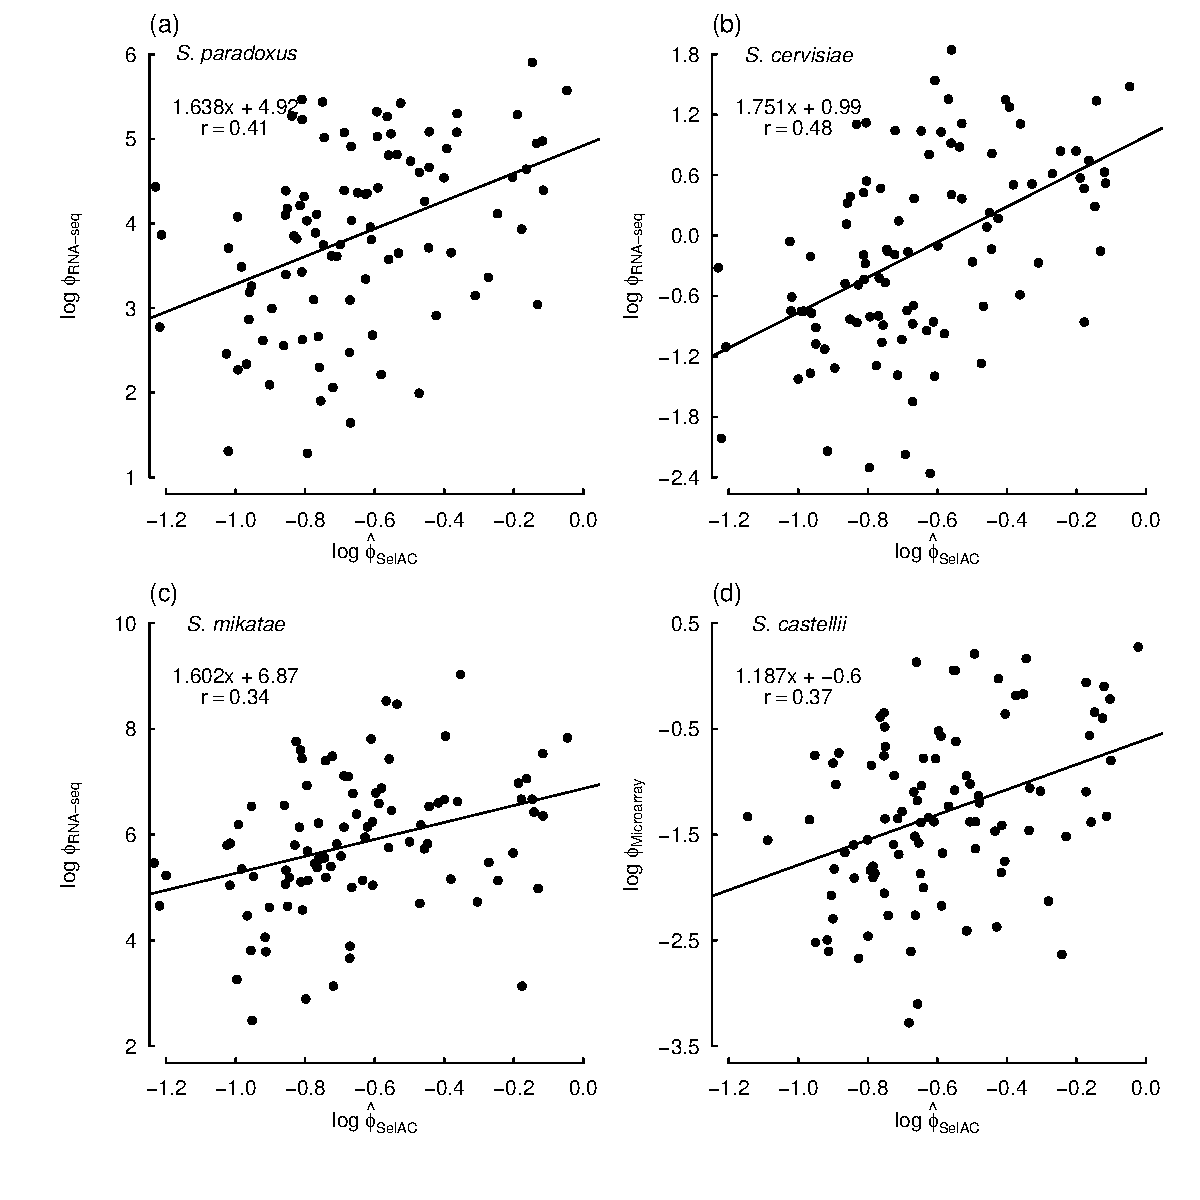
\includegraphics[width=0.9\linewidth]{FIGURE_1_SelACwG_vs_Empirical_by_spp.pdf}
  \caption{Comparisons between estimates of $\phi$ obtained from \selacplusgamma and direct measurements of expression for individual yeast taxa across the 100 selected genes from \citet{SalichosAndRokas2013}.
  	Estimates of $\phi$ were obtained by solving for $\psi$ based on estimates of $\psiprime$, and then dividing by \Funcaveci. 
  	Gene expression was measured using either RNA-Seq (a-c) or Microarray chips (d), and the equations in the upper left hand corner of each panel represent the regression fit and correlation coefficient $r$.
  } 
  \label{fig:PhivsEmpirical}
\end{figure}


\begin{figure}[H]
  \centering
  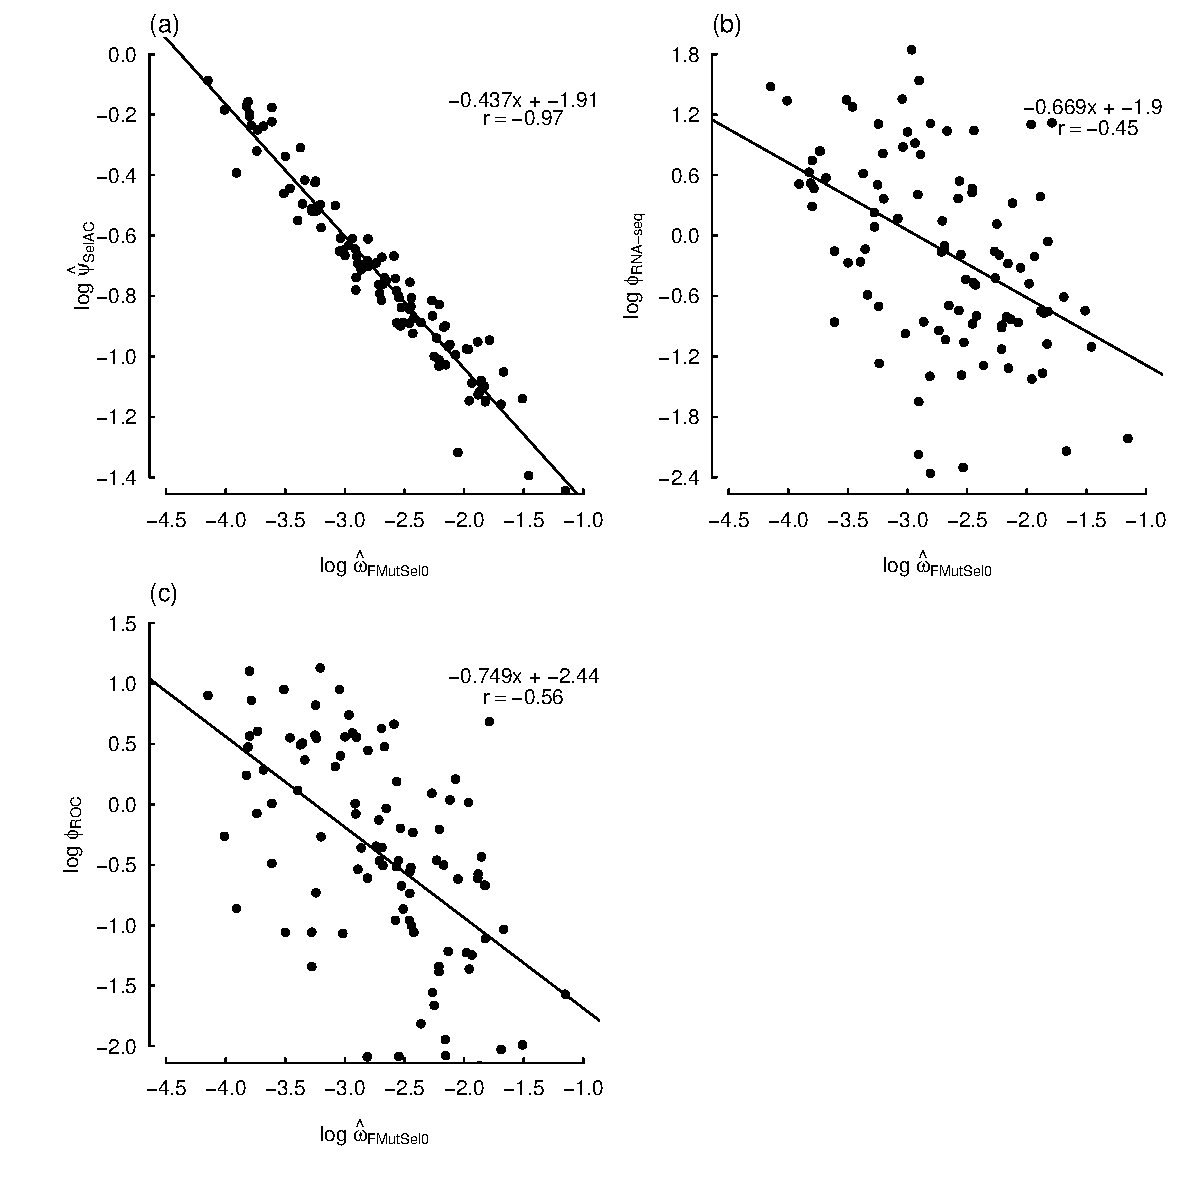
\includegraphics[width=0.9\linewidth]{FIGURE_2_MutSelOmega_vs_Us_ROC_Scer_only.pdf}
  \caption{Comparisons between $\omega$, which is the nonsynonymous/synonymous mutation ratio in FMutSel0, $\psi$ obtained from \selacplusgamma (a), a direct measurement of expression (b), and a model-based prediction of gene expression that does not account for ancestry (c), for \emph{S. cerevisiae} across the 100 selected genes from \citet{SalichosAndRokas2013}.  
    As in Figure \ref{fig:PhivsEmpirical}, the equations in the upper left hand corner of each panel provide the regression fit and correlation coefficient.
    Estimates of $\psi$ were solved from estimates of $\psiprime$.
  } 
  \label{fig:OmegavsPsi}
\end{figure}


\begin{figure}[H]
  \centering
  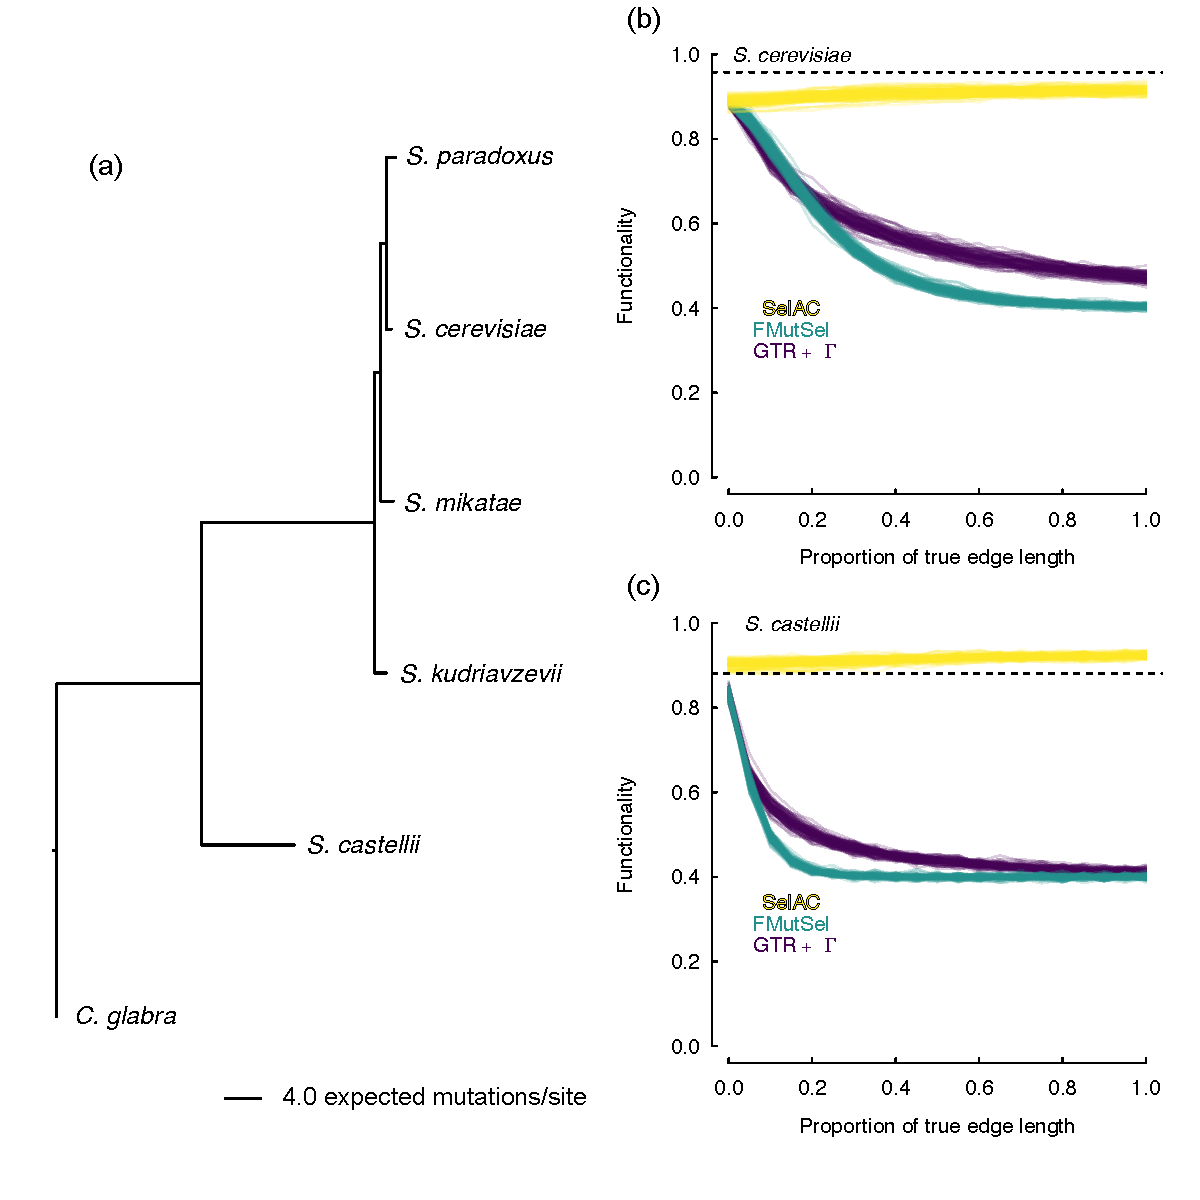
\includegraphics[width=0.9\linewidth]{FIGURE_3_Inferred_Tree_AND_Model_Adequacy.pdf}
  \caption{(a) Maximum likelihood estimates of branch lengths under \selacplusgamma for 100 selected genes from \citet{SalichosAndRokas2013}.  
    Tests of model adequacy for \emph{S. cerevisiae} (b) and \emph{S. castellii} (c) indicated that, when these taxa are removed from the tree, and their sequences are simulated, the parameters of \selacplusgamma exhibit functionality that is far closer to the observed (dashed black line) than data sets produced from parameters of either FMutSel0 or GTR + $\Gamma$. 
}
  \label{fig:TreeAndAdequacy}
\end{figure}


\clearpage

\setcounter{figure}{0}
\setcounter{table}{0}
\setcounter{page}{1}
\setcounter{section}{0}

\renewcommand{\thefigure}{S\arabic{figure}}
\renewcommand{\thetable}{S\arabic{table}}
\renewcommand{\thepage}{S\arabic{page}}
\renewcommand{\thesection}{\arabic{section}} %
\renewcommand{\appendixname}{Supporting Materials}
\renewcommand{\theequation}{S\arabic{equation}}

\setcounter{equation}{0}
\appendix
\part{\appendixname}
%Supporting Materials for \emph{\thetitle} \  by Beaulieu \emph{et al.}~(In Review).

\section{Supporting Materials}

\subsection{Comparisons of SelAC gene expression estimates with empirical measurements}

In our model, the parameter $\phi$ measures the realized average protein synthesis rate of a gene. 
We compared our estimates of $\phi$ to two separate measures of gene expression, one empirical (See Figure \ref{fig:PhivsROC}), and one model-based prediction that does not account for shared ancestry, for individual yeast taxa across the same set of genes. 
Our estimates of $\phi$ are positively correlated both measures, which are also strongly correlated with each other (Figure \ref{fig:PhivsEmpirical} - \ref{fig:ROCvsEmpirical}) 
On the whole, these comparisons indicate not only a high degree of consistency among all three measures, but also, importantly, that estimates of $\phi$ obtained from SelAC provide real biological insight into the expression level of a gene.

\begin{figure}[H]
  \centering
  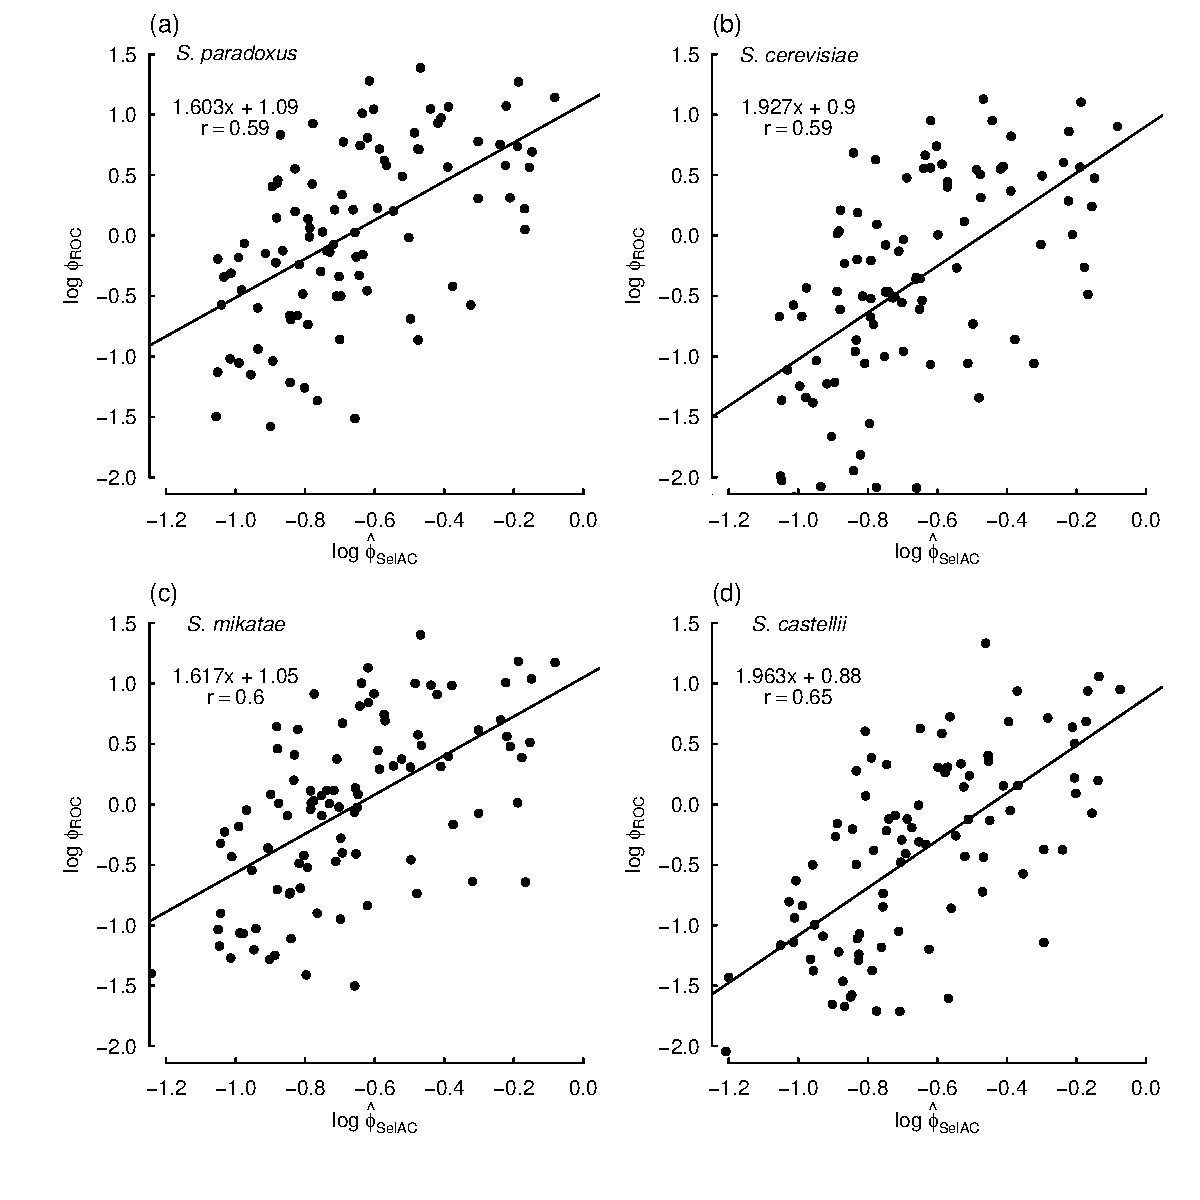
\includegraphics[width=0.9\linewidth]{FIGURE_S1_SelACwG_vs_ROC_by_spp.pdf}
  \caption{Comparisons between estimates of $\phi$ obtained from \selacplusgamma and the predicted gene expression from the ROC SEMPER model (\citet{GilchristEtAl2015}) for individual yeast taxa across the 100 selected genes from \citet{SalichosAndRokas2013}.
    	As with figures in the main text, estimates of $\phi$ were obtained by solving for $\psi$ based on estimates of $\psiprime$, and then dividing by \Funcaveci. 
  		The equations in the upper left hand corner of each panel represent the regression fit and correlation coefficient.
  } 
  \label{fig:PhivsROC}
\end{figure}


\begin{figure}[H]
  \centering
  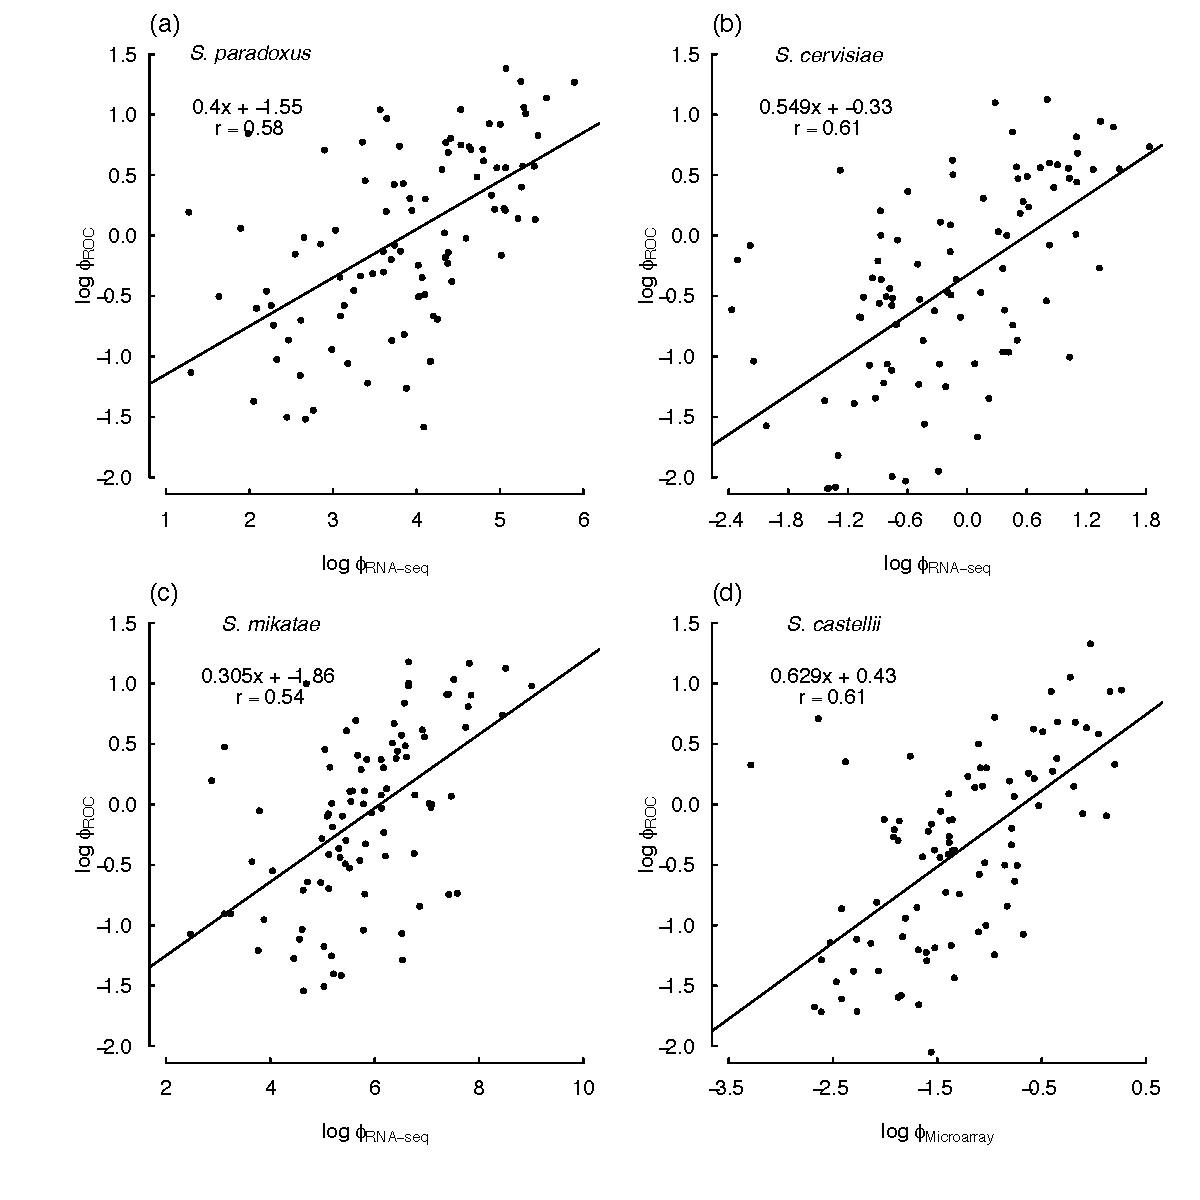
\includegraphics[width=0.9\linewidth]{FIGURE_S2_Empirical_vs_ROC_by_spp.pdf}
  \caption{Comparisons of predicted gene expression from the ROC SEMPER model (\citet{GilchristEtAl2015}) and direct measurements of expression from RNA-Seq or Microarray data for individual yeast taxa across the 100 selected genes from \citet{SalichosAndRokas2013}.
      	The equations in the upper left hand corner of each panel represent the regression fit and correlation coefficient.
  } 
  \label{fig:ROCvsEmpirical}
\end{figure}


\subsection{Simulations}

Overall, the simulation results indicate that SelAC model can reasonably recover the known values of the generating model (Figure \ref{fig:SelacNoGSimRes} - \ref{fig:SelacWithGSimRes2}).
This includes not only the parameters in the model, but also the optimal amino acids for a given sequence as well as the estimates of the branch lengths.
There are a few observations to note.
First, the ability to accurately recover the true optimal amino acid sequence will largely depend on the magnitude of $\phi$.
This is, of course, intuitive, given that $\phi$ sets the strength of stabilizing selection towards an optimal amino acid at a site.
However, the inclusion of $\alphag$ into the model, appears to generally increase values of $\phi$ and generally improves the ability to recover the optimal amino acids even for the gene with the lowest baseline $\phi$.
Second, we found a strong downward bias in estimates of $\alphag$, which actually translates to greater variation among the rate categories. 
The choice of a gamma distribution to represent site-specific variation in sensitivity was based on mathematical convenience and convention, rather than on biological reality.
Nevertheless, we suspect that this bias is in large part due to the difficulty in determining the baseline $\psi$ for a given gene and the value of $\alphag$ that globally satisfies the site-specific variation in sensitivity across all genes, as indicated by the slight upward bias in estimates of $\psi$.
It has been suggested, in studies of the behavior of the the gamma distribution in applications of nucleotide substitution model, that increasing the number of rate categories can often improve accuracy of the shape parameter (\citet{MayroseEtAl2005}).
Future work will address this issue.


\begin{figure}[H]
  \centering
  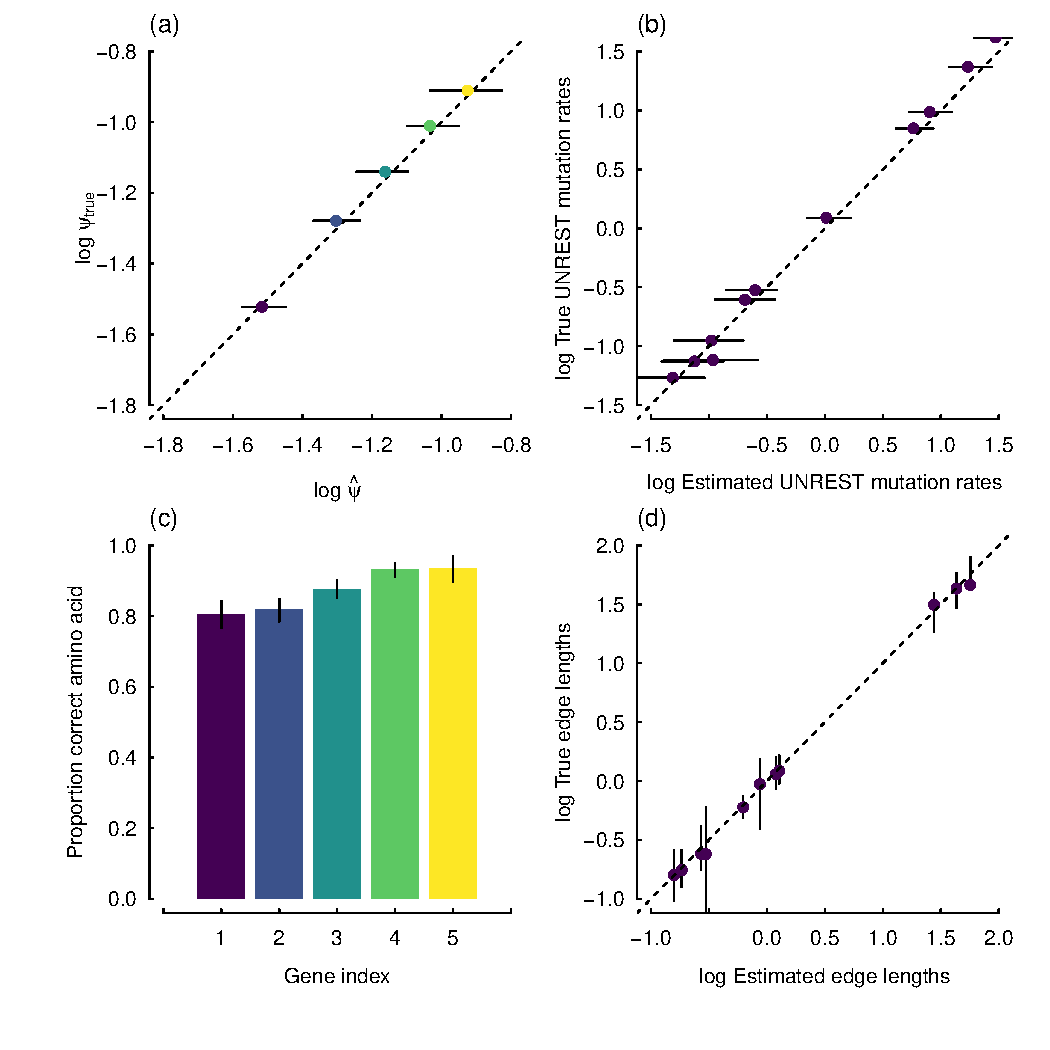
\includegraphics[width=0.9\linewidth]{FIGURE_S3_5genes_ALL_UNREST_Selac_NoG.pdf}
  \caption{Summary a 5-gene simulation for a SelAC model where we assume $\alphag = \infty$, and thus, no site-specific sensitivity in the generating model.
		The 'known' parameters were based on fitting the same SelAC to the 106 gene data set and phylogeny of \citet{RokasEtAl2003}, with gene choice being based on five evenly spaced points along the rank order of the gene specific composite parameter $\psiprime_g$.
		The points and associated uncertainty in the estimates of the gene-specific average protein synthesis rate, or $\psi$ (calculated from $\psiprime$)(a), nucleotide mutation rates under the UNREST model (b), proportion of correct optimal amino acids for a given gene (c), and estimates of the individual edge lengths are based the mean and 2.5\% and 97.5\% quantiles across on 50 simulated datasets.
} 
  \label{fig:SelacNoGSimRes}
\end{figure}

\begin{figure}[H]
  \centering
  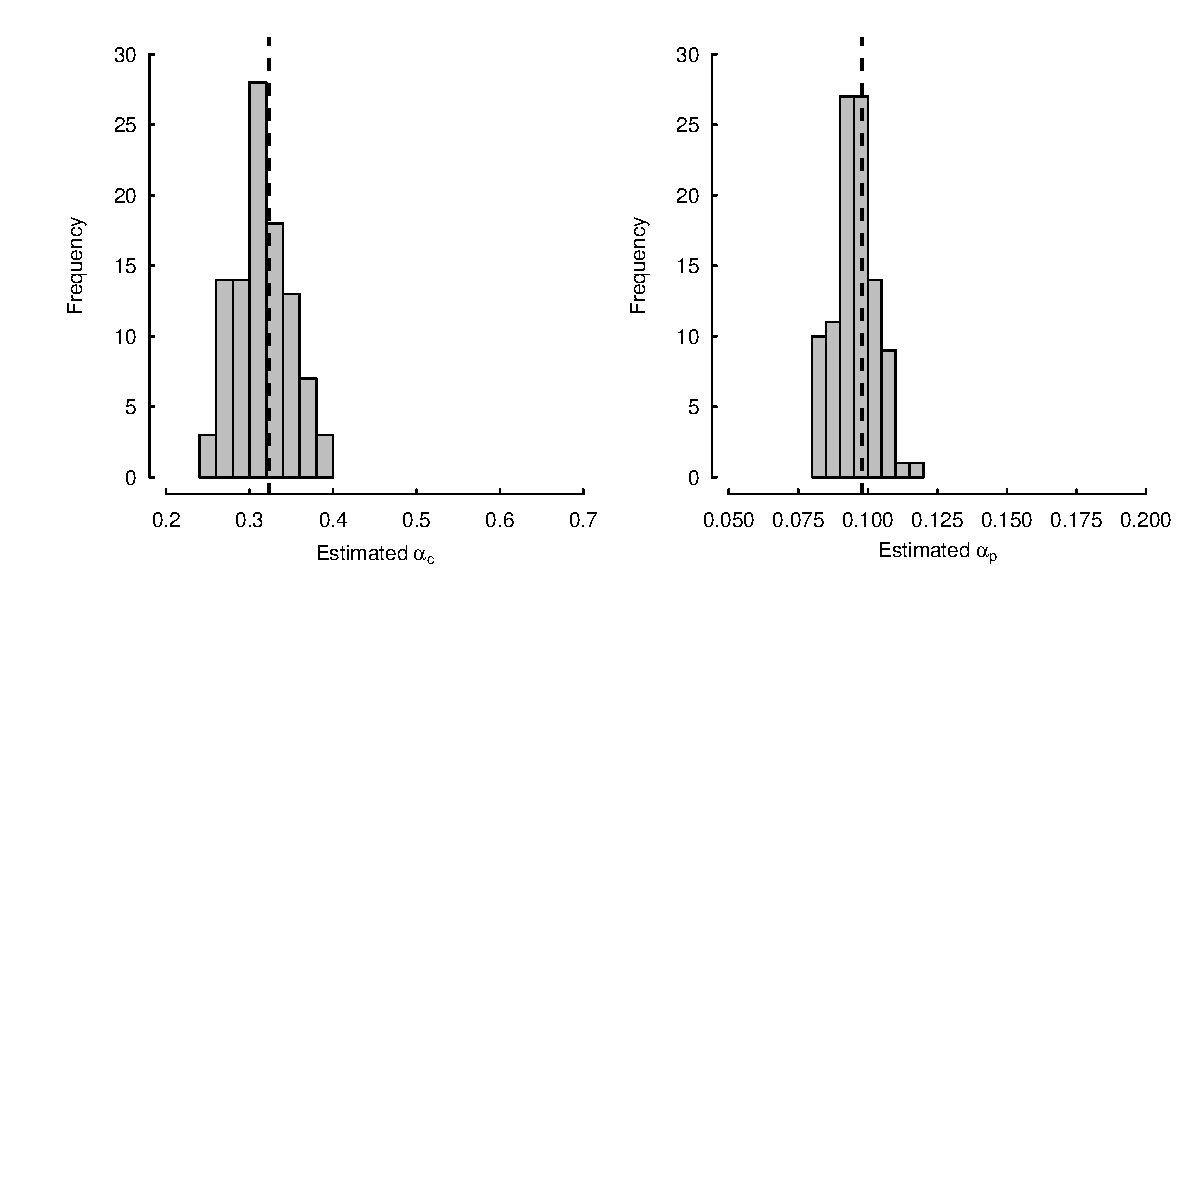
\includegraphics[width=0.9\linewidth]{FIGURE_S4_5genes_alpha_beta_UNREST_Selac_NoG.pdf}
  \caption{The distribution of estimates of the Grantham weights, $\alphac$ and $\alphap$, in a SelAC model, where we assume $\alphag = \infty$, and thus no site-specific sensitivity in the generating model.
  		The dashed line represents the value used in the generating model. 
  } 
  \label{fig:SelacNoGSimRes2}
\end{figure}

\begin{figure}[H]
  \centering
  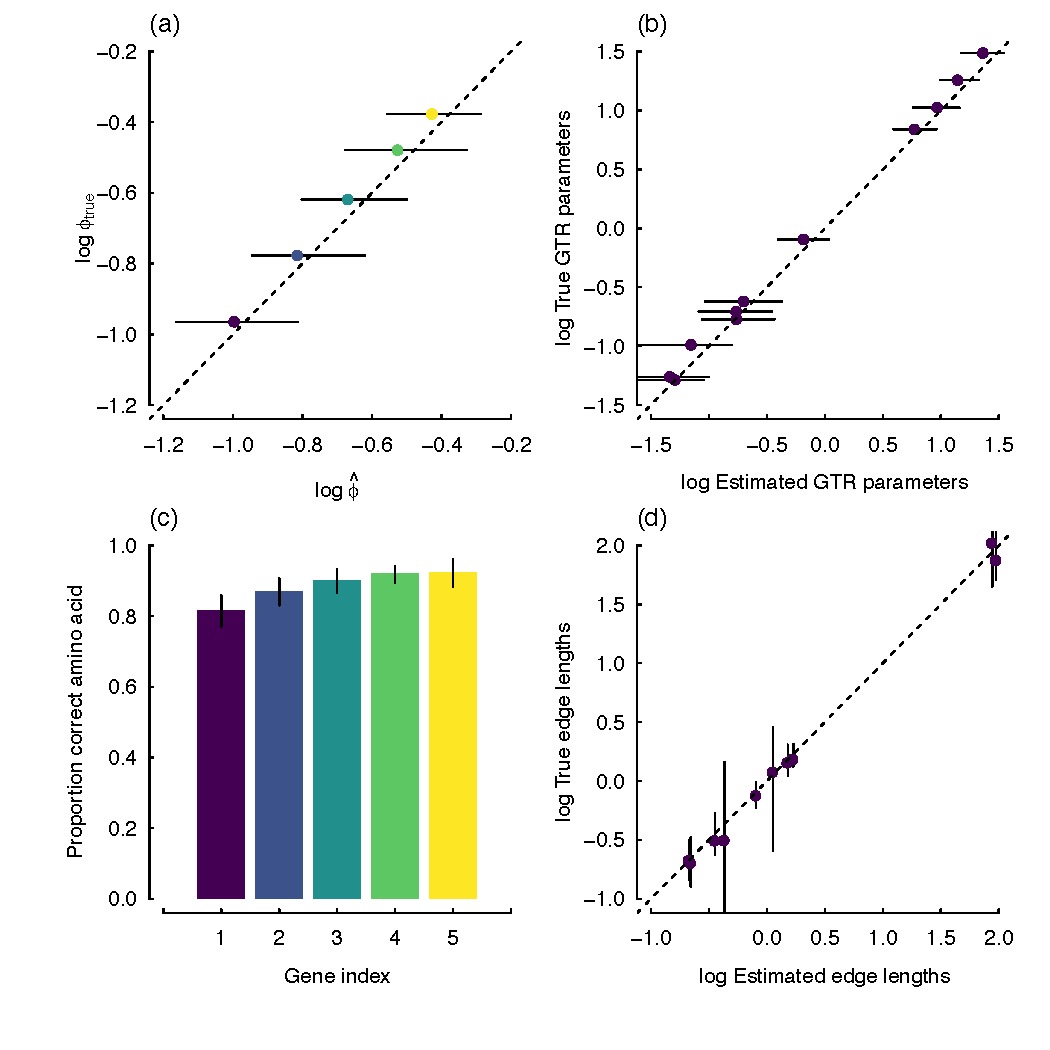
\includegraphics[width=0.9\linewidth]{FIGURE_S5_5genes_All_UNREST_WITHGAMMA.pdf}
  \caption{Same figure as in Figure S3, except the generating model includes site-specific sensitivity in the generating model (i.e., $\alphag$).
  } 
  \label{fig:SelacWithGSimRes}
\end{figure}

\begin{figure}[H]
  \centering
  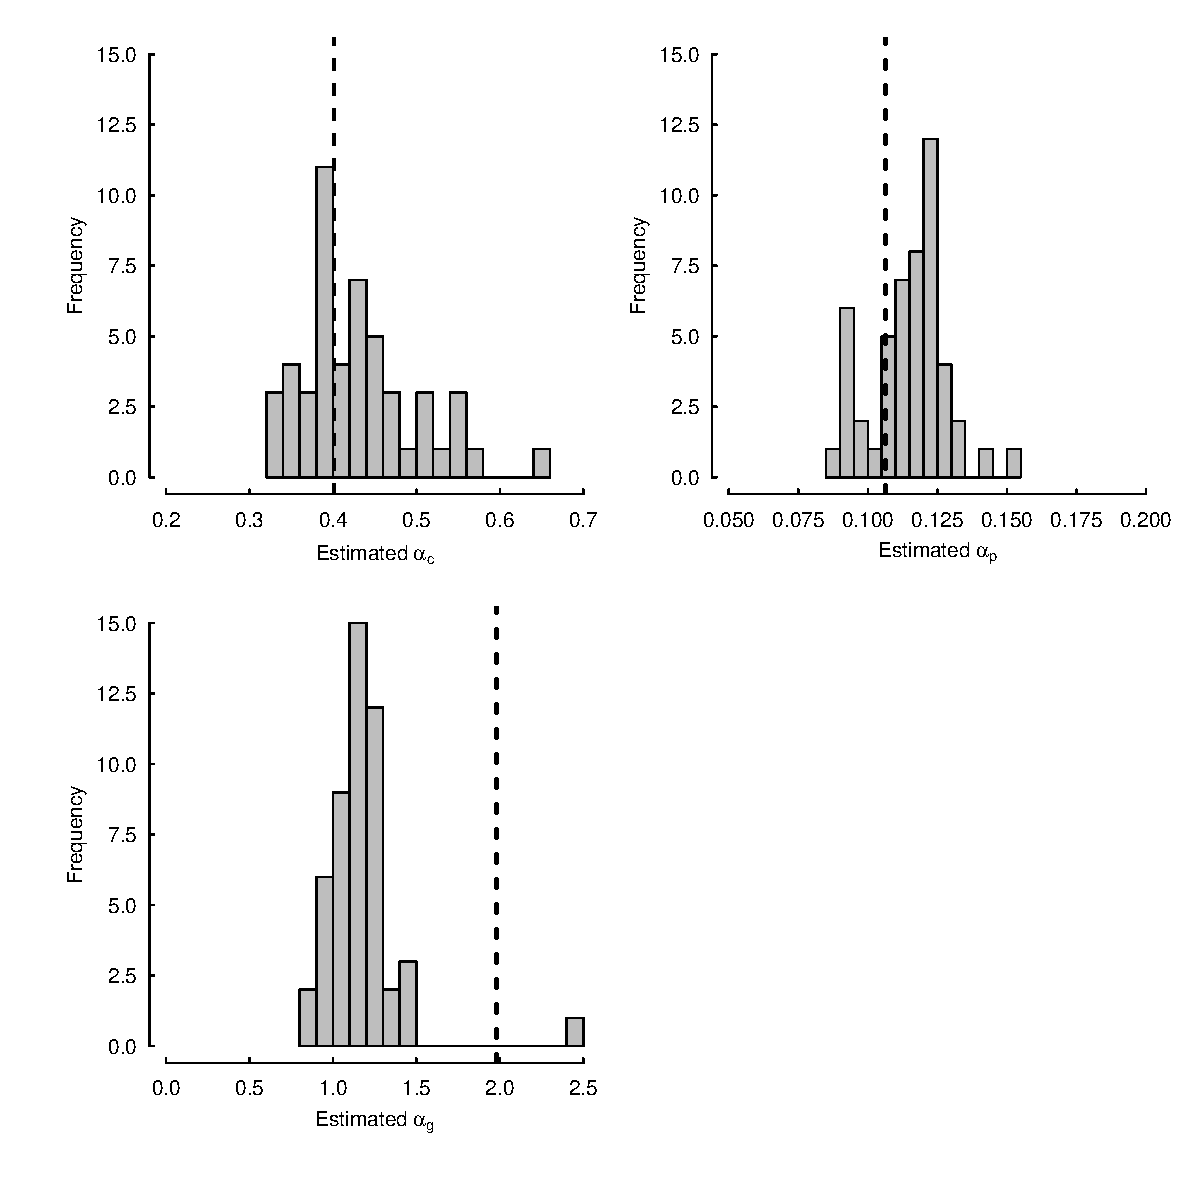
\includegraphics[width=0.9\linewidth]{FIGURE_S6_5genes_alpha_beta_gammashape_UNREST_WITHGAMMA.pdf}
  \caption{Same figure as in Figure S4, except the generating model includes site-specific sensitivity in the generating model (i.e., $\alphag$).
  		Unlike, Grantham weights, which showed no systematic bias, there is a downward bias in estimates of $\alphag$.
  } 
  \label{fig:SelacWithGSimRes2}
\end{figure}


\end{document}
